\documentclass[a4paper,11pt,twocolumn,unpublished]{quantumarticle}
\pdfoutput=1

\usepackage{graphicx}
\usepackage{amsmath,amssymb}
\usepackage{bm}
\usepackage{braket}
\usepackage{booktabs}
\usepackage[numbers,sort&compress]{natbib}
\usepackage{nameref}

\graphicspath{{../../results/}}

\newcommand{\CR}{\mathcal{C}_R}
\newcommand{\Ic}{I_c}
\newcommand{\Ztwo}{\mathbb{Z}_2}

\begin{document}

\title{Scrambling, not athermality, protects quantum information under generic
measurement: chaotic states outperform quantum many-body scar codes}

\author{Hikaru Wakaura}
\orcid{0000-0001-8381-8323}
\email{h.wakaura@qiri.co.jp}
\affiliation{QIRI (Quantum Integrated Research Institute Inc.), Tokyo 107-0061, Japan}
\author{Taiki Tanimae}
\email{t.tanimae@qiri.co.jp}
\affiliation{QIRI (Quantum Integrated Research Institute Inc.), Tokyo 107-0061, Japan}

\maketitle

\begin{abstract}
% (1) introduction — all-fields scientist
Monitored quantum many-body systems protect quantum information from projective
measurements exactly when their unitary dynamics scramble it, placing the
measurement-induced transition on the same footing as quantum error correction.
% (2) background — related-field scientist
Because the eigenstate thermalization hypothesis endows chaotic eigenstates with
approximate Knill--Laflamme structure, it is natural to ask whether quantum
many-body scars---non-thermal eigenstates that stay weakly entangled and
dynamically coherent---form especially good codes.
% (3) problem
Whether they protect information better or worse than the surrounding thermal
states has not been settled quantitatively.
% (4) main result — "Here we show" (design principle fronted)
Here we show that scrambling, not athermality, is what protects an encoded
qubit: under monitored dynamics, the reference-qubit coherent information of a
logical qubit encoded in the PXP scar subspace lies below that of an
energy-matched thermal encoding for every measurement we test.
% (5) comparison with prior work
The deficit is mild for local measurement, largest for collective measurements
aligned with the emergent $\mathrm{su}(2)$ order parameter that couples the code
states, and survives a fine-tuned Casimir measurement for which the scar code
is a nominal decoherence-free subspace: at every rung the scars carry excess
Casimir variance over thermal neighbors, and the deficit tracks that excess.
% (6) generalized meaning
An exactly solvable spin-1 model isolates that variance as the control
parameter: only zero-variance \emph{exact} scars are protected, and their
local-measurement advantage decays with rate, its large-size fate open. The
eigenstate-thermalization-to-error-correction correspondence thus holds directly
in the monitored-circuit setting, and approximate scarring does not aid
protection against generic measurement.
% (7) broad outlook
Scrambling is therefore the design resource for measurement-robust encoding, and
weak-ergodicity-breaking subspaces are liabilities rather than assets for
measurement-based quantum memories.
\end{abstract}

\section{Introduction}

% 大: broad topic everyone cares about
The competition between scrambling unitary dynamics and local measurements
drives a sharp transition in how much quantum information a many-body system
retains~\cite{Li2018MIPT,Li2019,Skinner2019,Chan2019,Bao2020,Jian2020,Fisher2023}. This measurement-induced phase
transition (MIPT) is now understood as a coding transition: below a critical
measurement rate the dynamics act as an emergent quantum error-correcting code
that hides logical information non-locally, protecting it from measurements that
act as erasure errors~\cite{Choi2020,Gullans2020,Fan2021}. The order parameter
is information-theoretic---the coherent information, or equivalently the
entanglement of a reference qubit maximally entangled with the encoded
information~\cite{Gullans2020,Gullans2020b,Qian2024}.

% 中: narrowing toward the specific question
The coding power of chaotic dynamics is inherited by chaotic \emph{eigenstates}.
The eigenstate thermalization hypothesis (ETH) forces local operators to have
smooth diagonal and exponentially small off-diagonal matrix
elements~\cite{Deutsch1991,Srednicki1994,Rigol2008,DAlessio2016}, which is
exactly the approximate Knill--Laflamme condition~\cite{KnillLaflamme1997};
thermal eigenstates therefore form approximate codes whose error scales with the
system's chaoticity~\cite{Brandao2019,BaoCheng2019,Qasim2025}. Quantum many-body scars are the
conspicuous exception to ETH: a measure-zero tower of atypically weakly
entangled, dynamically reviving eigenstates embedded in an otherwise thermal
spectrum~\cite{Bernien2017,Turner2018,Turner2018b,Serbyn2021,Moudgalya2022}.
Scars can be embedded in decoherence-free
subspaces~\cite{Zanardi1997,Lidar1998,WangDFS2024}, and projective measurement can
even enhance their revivals~\cite{Paviglianiti2025}, suggesting they might be
privileged carriers of quantum information under monitoring.

% 小 + However (only once) + In this study
However, whether a logical qubit stored in the scar subspace is protected better
or worse than one stored in the surrounding thermal bulk---at matched energy, in
the same monitored dynamics, quantified by the coherent information the
monitored channel retains---has not been determined. In this study, we compute
the reference-qubit coherent information $\CR$ of scar and thermal codes of the
monitored PXP chain across local, collective, and Casimir measurement models. We find that thermal codes protect
information better than scar codes in every case; that an apparent scar advantage
seen against a single thermal reference is an artifact of an atypical baseline
and vanishes under ensemble averaging; and that the scar's emergent-$\mathrm{
su}(2)$ structure is a liability, not a shield, because its generator couples the
code states and the scars' excess Casimir variance defeats even a fine-tuned
decoherence-free encoding.

% 大: impact
The result establishes the ETH-to-error-correction correspondence as an operational
statement about monitored circuits and removes weak-ergodicity-breaking subspaces
from the menu of candidate measurement-robust quantum memories.

\section{Model and diagnostics}

\subsection{Model, encoding, and monitored dynamics}

We study the PXP chain of $L$ sites in the Rydberg-blockaded (constrained)
Hilbert space of dimension $F(L{+}2)$ (Fibonacci), with
\begin{equation}
H = \sum_i P_{i-1}\, X_i\, P_{i+1}, \qquad P=\ket{0}\bra{0},
\end{equation}
whose $\Ztwo$ N\'eel state exhibits the canonical scar
revivals~\cite{Bernien2017,Turner2018,Lin2019,Ho2019} (period
$t\simeq4.7$, fidelity $\simeq0.74$ at $L=12$). We identify the $L{+}1$ scar-tower
eigenstates by their anomalous overlap with $\ket{\Ztwo}$.

A logical qubit is encoded in a two-dimensional subspace
$\{\ket{0_L},\ket{1_L}\}$ and maximally entangled with a reference $R$,
$\ket{\Psi_0}=(\ket{0}_R\ket{0_L}+\ket{1}_R\ket{1_L})/\sqrt2$. The system
evolves by alternating steps of PXP evolution $e^{-iH\,dt}$ and random projective
measurement; per quantum trajectory the joint state stays pure and the reference
entanglement entropy $S_R=-\mathrm{Tr}\,\rho_R\log_2\rho_R\in[0,1]$ measures the
surviving logical information. Its trajectory average
\begin{equation}
\CR(p) = \big\langle S_R \big\rangle_{\text{traj}}
\end{equation}
is the single-qubit coherent information of the monitored channel at fixed
circuit depth: $\CR\to1$ recoverable, $\CR\to0$ lost. Concretely we run $40$
evolution--measurement steps and estimate $\CR$ as the time average of $S_R$
over the last quarter of the record ($t\in[21.6,24]$). In a finite system at
$p>0$ every code eventually purifies, so $\CR$ is a fixed-depth retained
information, not an asymptotic capacity; what we compare is the scar--thermal
\emph{ordering} at matched depth, which is depth-robust---doubling and
quadrupling the depth leaves the collective-channel deficit essentially
unchanged ($-0.27$, $-0.34$, $-0.33$ at depths $40$, $80$, $160$, $L{=}14$,
$p{=}0.10$) while both codes decay (Appendix~\ref{app:algorithm}). We take
$dt=0.6$ and measurement probability $p$ per site (local) or per operator
(collective) per step. To control the
energy-mismatch confound, thermal codes are drawn from generic eigenstates
energy-matched to the two scar-rung energies within a tolerance $\pm0.5$
(realized offsets at $L{=}14$: $0.22$ on average, $0.47$ at most);
\textbf{the thermal baseline is averaged over an ensemble of $\sim\!10$--$20$
such pairs}, without which a single atypical pair inverts the conclusion
(Sec.~\ref{sec:results}). The comparison is insensitive to this tolerance:
tightening the window to $\pm0.1$ leaves the scar deficit unchanged, and
within the ensemble $\CR$ is uncorrelated with the residual offset
(Appendix~\ref{app:ensemble}).

We study $L=10$--$18$ (constrained dimension up to $F(20)=6765$) with $40$
evolution--measurement steps per trajectory and average $\CR$ over $120$--$400$
Born-sampled quantum trajectories. Reported statistical error bars are the
standard error of the mean over trajectories; the thermal band is the standard
deviation of $\CR$ over the ensemble of energy-matched thermal pairs. All runs
use fixed random seeds and are reproducible from the accompanying code.

Statically we probe the Knill--Laflamme violation of a code under an error set
$\{E_a\}$ through the logical leak $\langle 0_L|E_a|1_L\rangle$ and the
distinguishability $\langle0_L|E_a|0_L\rangle-\langle1_L|E_a|1_L\rangle$.

\subsection{A model-independent criterion}
\label{sec:criterion}
A projective measurement of a Hermitian operator $O$ leaves the encoded qubit
literally untouched only if the code is an eigenspace of $O$ with a single
shared eigenvalue; more generally, the qubit survives a single shot if and only
if the Knill--Laflamme conditions hold for the projector set $\{\Pi_g\}$ of
$O$'s eigenspaces~\cite{KnillLaflamme1997}. A measurement \emph{resolves}---and
hence degrades---the code through two channels: \emph{(i) eigenvalue
distinguishability}, when the two logical states' outcome distributions
$P_a(g)=\langle a_L|\Pi_g|a_L\rangle$ differ; and \emph{(ii) non-invariance},
when a sector-restricted overlap $\langle0_L|\Pi_g|1_L\rangle$ is nonzero,
coherently mixing the logical states. Equal means and a vanishing global leak
$\langle0_L|O|1_L\rangle$ are therefore insufficient: a code spread over many
$O$-sectors---a large $O$-variance---is collapsed by the shot, and survival then
requires the sector-wise conditions in \emph{every} occupied sector, which is
why a true decoherence-free subspace demands logical states that are
$O$-eigenstates sharing one eigenvalue. This criterion is independent of the
microscopic model and organizes the results below: thermal states, spread
broadly and near-identically in a local basis, are close to optimal codes,
while scars are penalized whenever the measured operator resolves their
atypical structure. Both channels combine into a single exact, simulation-free
scalar---the reference entropy $s_1(O)$ surviving one $O$-measurement, which
equals unity precisely when the sector-wise conditions hold---and $s_1$
predicts the monitored $\CR$ across resolving measurements
(Appendix~\ref{app:predictor}).

A scoping remark on vocabulary. Throughout, ``scrambling'' refers to the
structural imprint of chaotic dynamics on \emph{eigenstates}---the ETH
matrix-element structure that spreads a code broadly and near-identically
over the measured operator's eigenbasis---not to dynamical operator growth
during the monitored evolution: for eigenstate codes the unitary acts
trivially (up to a relative phase) on the code subspace between measurements,
so protection is a property of how the measurement resolves the code, exactly
the two channels above. We neither measure dynamical chaos diagnostics
(out-of-time-order correlators, level statistics) nor tune chaoticity
independently of the code; ``scrambling versus athermality'' is operational
shorthand for ETH-typical versus scar-atypical eigenstate structure with
respect to the measured operator.

\section{Results}
\label{sec:results}

\subsection{Thermal codes win: the apparent scar advantage is a baseline artifact}
Figure~\ref{fig:crossover} compares $\CR(p)$ for the scar code against the
thermal ensemble. For both local-$Z$ and collective (staggered-$Z$) monitoring
the scar curve lies below the thermal-ensemble mean at every $p>0$, and below
the $\pm1\sigma$ ensemble band at every $p>0$ for the collective channel and
for $p\le0.12$ for the local one (at $p=0.14$, $0.16$ both codes are nearly
purified, $\CR<0.03$, and the residual gap is within the band). A single
nearest-in-energy thermal pair sits at the $0$th percentile of the ensemble
($\CR=0.53$ versus ensemble mean $0.87$ at $L{=}14$, $p{=}0.10$, collective),
which is why an unaveraged comparison spuriously favors the scar.

\begin{figure}[t]

\includegraphics[width=\linewidth]{corrected_crossover.pdf}
\caption{\textbf{Thermal codes protect information better than scar codes.}
Reference-qubit coherent information $\CR$ versus measurement rate $p$ for the
scar code (red) and the thermal ensemble (blue; band is $\pm1\sigma$ over the
ensemble) under (a) local-$Z$ and (b) collective staggered-$Z$ monitoring
at $L=14$. The scar lies below the thermal mean at every $p>0$, and below the
band except at the largest local rates, where both codes are nearly purified.}
\label{fig:crossover}
\end{figure}

\subsection{The disadvantage persists to the largest accessible size}
Figure~\ref{fig:scaling} shows $\Delta\CR\equiv\CR^{\rm scar}-\langle\CR^{\rm
therm}\rangle$ at $p=0.10$. It is negative for all $L=10$--$18$ and both
channels: $-0.008$ to $-0.06$ (local) and $-0.25$ to $-0.32$ (collective). The
thermal-ensemble band excludes zero at every size for the collective channel,
and at every size except $L=12$ for the local one (there $-0.008\pm0.009$,
consistent with zero). At the largest size $L=18$ (constrained dimension
$6765$) the gap is $-0.05$ (local) and $-0.30$ (collective), the collective gap
essentially size-independent: the refutation is not a finite-size artifact.

\begin{figure}[t]
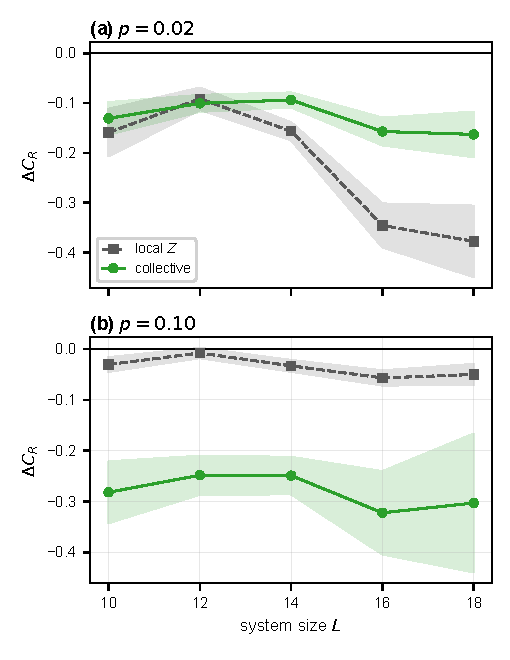
\includegraphics[width=\linewidth]{ensemble_scaling.pdf}
\caption{\textbf{The scar disadvantage $\Delta\CR<0$ at every size.} Scar-minus-thermal
coherent information at $p=0.10$ versus $L$ for local (grey) and
collective (green) monitoring; shading is the thermal-ensemble spread
($12$ pairs, $200$ trajectories for $L=10$--$16$; $6$ pairs, $120$
trajectories for $L=18$).}
\label{fig:scaling}
\end{figure}

\subsection{Even the maximal scar code loses}

We emphasize that this single-qubit comparison is the most favorable one for the
scar: the scar tower is only $(L{+}1)$-dimensional, so it can host at most
$\log_2(L{+}1)$ logical qubits---a sub-extensive capacity, against the
exponentially large thermal bulk. A scar subspace therefore cannot support an
extensive code even before dynamics; the per-qubit comparison already settled
here is its best case, and it loses. That best case is moreover robust to the
choice of rungs: scanning \emph{every} pair of positive-energy tower rungs at
$L=10$ and $14$, even the best-performing pair lies below the
thermal-ensemble mean in both channels (at $L=14$, best $0.081$ versus
thermal $0.099$ local and $0.784$ versus $0.865$ collective at $p=0.10$;
\texttt{scripts/referee\_audit.py}), so the deficit is a property of the
tower, not of the canonical pair.

To confirm this directly, we encode the \emph{maximal} scar code---all
$k=\lfloor\log_2(L{+}1)\rfloor$ logical qubits, i.e. $2^k$ tower states
maximally entangled with a $k$-qubit reference---and compare its
protected-information density $S_R/k$ against a same-dimension thermal code under local
monitoring (Fig.~\ref{fig:ext}). The scar loses at every rate: at $L=14$
($k=3$), $\Delta(S_R/k)=-0.17,-0.14,-0.06$ at $p=0.02,0.04,0.08$, with the
thermal ensemble tightly determined ($\sigma\lesssim0.01$), and the gap persists
across $L=10,14,18$. The gap is even larger under collective staggered-$Z$
monitoring ($\Delta(S_R/k)=-0.32$ to $-0.43$ at $L=14$), while under the
fine-tuned Casimir $J^2$ the two codes are comparable ($|\Delta|\lesssim0.03$;
Appendix~\ref{app:extensive})---the same exception seen in the single-qubit and
spin-1 analyses. Even the largest code the scar subspace admits is thus a worse
monitored memory than a generic thermal code of equal size under any generic
measurement.

\begin{figure}[t]

\includegraphics[width=\linewidth]{extensive.pdf}
\caption{\textbf{The maximal scar code loses even as an extensive memory.}
Protected-information density $S_R/k$ for the maximal $k=\lfloor\log_2(L{+}1)
\rfloor$-qubit scar code (solid) and a same-dimension thermal code (dashed,
$\pm1\sigma$ band) versus $p$ under local monitoring, for $L=10,14,18$. Scar
lies below thermal throughout.}
\label{fig:ext}
\end{figure}

\subsection{Mechanism: both channels resolve the scar code}
The PXP scar realizes both channels of the criterion while thermal codes realize
neither. Channel (ii) dominates under the collective staggered operator
$M=\sum_i(-1)^iZ_i$---the staggered magnetization, order parameter of the
emergent $\mathrm{su}(2)$ scar dynamics~\cite{Choi2019}---which carries a large
logical leak
$|\langle0_L|M|1_L\rangle|=1.73$ between the scar rungs (versus $\approx0$ for
thermal codes) and coherently mixes them. This leak is a one-sided suppressor of
$\CR$ [Fig.~\ref{fig:mech}(b)]: every high-leak code is poorly protected,
whereas low leak permits any value. Channel (i)---eigenvalue distinguishability
through $O$-variance---is isolated by the Casimir measurement below. Accompanying
both is a weak monotone trend [Fig.~\ref{fig:mech}(a)]: protection rises with
the code's spread in the measurement basis, as ETH predicts, so that unstructured
thermal codes are close to optimal.

\begin{figure}[t]

\includegraphics[width=\linewidth]{mechanism.pdf}
\caption{\textbf{What controls collective protection.} Collective $\CR$ versus
(a) $Z$-basis participation and (b) logical leak $|\langle0|O|1\rangle|$
over an eigenstate sweep (blue), product states (orange), and the
canonical scar (star). Higher participation raises $\CR$; large leak suppresses
it. The scar is a low-$\CR$ outlier on both axes.}
\label{fig:mech}
\end{figure}

The full $(p,\ell)$ dependence, with $\ell$ the measurement support size
(block-sum of $\ell$ sites; $\ell{=}1$ local, $\ell{=}L$ global), is negative
throughout: the scar never wins (Fig.~\ref{fig:supp_pd},
Appendix~\ref{app:phasediagram}).

\subsection{The decoherence-free-subspace rescue fails at every rung}
\label{sec:dfs}
A true DFS~\cite{Zanardi1997,Lidar1998} for the scar code would restore an
advantage. The emergent Casimir
$J^2=\tfrac12(H^+H^-+H^-H^+)+J_z^2$, built from the exact split
$H=H^++H^-$~\cite{Choi2019},
gives the chiral-symmetric scar pair $(\ket{+E},\ket{-E})$ equal expectation and
vanishing leak ($\Delta\langle J^2\rangle=0.000$, leak $=0.052$ at the
canonical rung)---a nominal DFS.
Yet under $J^2$ monitoring the scar code still loses, $\Delta\CR=-0.18,-0.13,
-0.09$ at $p=0.04,0.08,0.12$ (about twice the ensemble spread; an independent
rerun with different seeds gives $-0.10,-0.08,-0.06$, so the sign is robust
while the magnitude fluctuates with the $10$-pair ensemble). The reason is
that equal expectation and zero leak
are necessary but not sufficient: a genuine DFS requires the code states to be
\emph{eigenstates} of the measured operator, and scar eigenstates carry
Casimir variance ($\mathrm{Var}\,J^2=32.5$ at the canonical rung, against
$5.5$ on average, range $2$--$17$, for the $19$ distinct energy-matched
thermal states).

That variance is not a fixed property of scarring but a hybridization
diagnostic---and scanning it across the tower turns the single failure above
into a controlled, intra-model test of the mechanism. The exact eigenstates
closest to the FSA rungs carry FSA weight $0.27$--$0.97$ and
$\mathrm{Var}\,J^2$ from $47.6$ down to $0.89$, decreasing monotonically from
the spectral center to the edge (Appendix~\ref{app:spectrum}); the canonical
rungs are the \emph{most} hybridized. Crucially, at every energy-matchable
rung the scar eigenstate retains \emph{excess} variance over its
energy-matched thermal neighbors [ratio $\simeq4.2$, $4.0$, $4.3$, $2.5$,
$1.6$ at $E\simeq2.7$, $4.1$, $5.3$, $6.6$, $7.7$], and the chiral pair at
every rung still loses under $J^2$ monitoring---$\Delta\CR<0$ throughout,
shrinking from $-0.16$ toward $-0.01$ as the excess variance shrinks
(\texttt{scripts/pure\_rung\_dfs.py}). The Casimir DFS thus fails
tower-wide, and the size of its failure tracks the scar's excess Casimir
variance---the quantity the exactly solvable model below tunes identically
to zero.

\subsection{A second model isolates the variance as the culprit}
To test generality and to isolate this mechanism we repeat the analysis in the
spin-1 Schecter--Iadecola magnet~\cite{Schecter2019}, whose scar tower
$\ket{S_n}=(Q^+)^n\ket{\Omega}$, $Q^+=\sum_j(-1)^j(S_j^+)^2$, is an \emph{exact}
su(2) multiplet. Two facts then hold to machine precision: the scars are exact
eigenstates, and the Casimir $J^2$ is exactly constant on the tower with
\emph{zero} variance on every scar---against $\mathrm{Var}\,J^2\simeq32$ for PXP
[Fig.~\ref{fig:spin1}(b)]. This flips the Casimir rescue
[Fig.~\ref{fig:spin1}(a)]: the exact-su(2) scar code is now a genuine
decoherence-free subspace---its two logical states are identical $J^2$
eigenstates, so a $J^2$ shot acts as the identity on the code and
$\CR^{\rm scar}=1$ at every $p$ \emph{by construction}
($\Delta\CR=+0.6$ to $+0.9$ against the thermal ensemble, $L=6,8$). The
content of this exactly solvable limit is therefore not the protection
itself but the contrast: the nominal DFS conditions that failed for PXP
(equal expectation, zero leak) here come with zero variance, and protection
is restored---completing, together with the intra-PXP rung scan of
Sec.~\ref{sec:dfs}, the case that the variance, not scarring itself,
controls the rescue. This is parameter-independent: for $(h,D)=(0.5,0.3)$ and
$(1.5,0.0)$ the Casimir variance again vanishes identically and $\CR^{\rm
scar}=1$ under $J^2$. Under generic local $S^z$ monitoring, by contrast, the
exact-scar code shows a low-rate scar-favorable difference whose behavior is
size-dependent, and we report it in full. At $L=6$ ($20$ thermal pairs) it
decays and changes sign within our window
($\Delta\CR=+0.10,+0.06,-0.02$ at $p=0.04,0.08,0.12$), as it does in two of
three parameter sets; at $L=8$ ($20$ pairs) it is larger and remains positive
throughout ($\Delta\CR=+0.20,+0.10,+0.08$, ensemble SEM $0.05$--$0.07$).
The same low-rate pattern appears in PXP at its purest rungs
($\Delta\CR\simeq+0.13$ at $p=0.04$ for the $E\simeq\pm6.6$ chiral pair,
decaying to $0$ by $p=0.12$; Sec.~\ref{sec:dfs}), with the caveat that
energy-matched partners near the spectral edge are themselves atypical. Two
sizes cannot settle whether this local advantage of \emph{exact} scars
survives at scale; what is settled is that it decays with rate and that no
such advantage exists for the hybridized PXP scar code that experiments
realize (Appendix~\ref{app:spin1}).

\begin{figure}[t]

\includegraphics[width=\linewidth]{spin1_rescue.pdf}
\caption{\textbf{Exact-su(2) scars evade the Casimir-variance obstruction.}
Second model (spin-1 Schecter--Iadecola, $L=6$, $20$-pair thermal ensemble).
(a) Scar$-$thermal coherent information $\Delta\CR$ versus $p$ (error bars are
the ensemble SEM). Under $J^2$ monitoring PXP scars lose (blue) while exact
spin-1 scars win perfectly (red); under generic local $S^z$ the exact-scar and
thermal codes are comparable at this size ($|\Delta\CR|\le0.1$, grey; at
$L=8$ the low-rate difference is larger, $+0.20$ at $p=0.04$, see text). (b) Scar
Casimir variance, $\simeq32$ (PXP, canonical rungs; $3.4$--$47.6$ across the
tower, always above energy-matched thermal neighbors) versus $\sim10^{-13}$
(exact) on a log scale---the control parameter of the rescue.}
\label{fig:spin1}
\end{figure}

\subsection{Relation to prior monitored-scar work}
Our protocol maps to the continuous-time rate of
Ref.~\cite{Paviglianiti2025} via $\gamma=p/dt$, so the range studied here
($p\le0.16$, $\gamma\le0.27$) brackets their critical rate
$\gamma_c\simeq0.013\pm0.002$ from above. We emphasize that at our sizes and
circuit depths the monitored-N\'eel entanglement density \emph{decreases} with
$L$ at every $p$ (Appendix~\ref{app:gamma}), i.e.\ we do not resolve the
volume-law phase or its critical point, and we therefore make no quantitative
comparison of critical rates; a minimum-spread estimate places the
steepest-variation scale at $p\sim0.05$ ($\gamma\sim0.08$), consistent in
order of magnitude but grid- and estimator-sensitive.

\subsection{Experimental accessibility}
The negative result is testable on the platform where PXP scars were first
observed~\cite{Bernien2017}. Programmable Rydberg-atom arrays natively realize
the blockaded dynamics, local-$Z$ monitoring is site-resolved projective
readout interleaved at a tunable rate, and the sizes studied here ($L\le18$)
are modest by current standards. Encoding in the scar subspace is accessible
through the N\'eel revival manifold, and the retained coherence can be
estimated by interferometric or randomized-measurement protocols. While
preparing individual thermal eigenstates is impractical, thermal-like codes can
be prepared operationally by pre-scrambling product states under the chaotic
dynamics itself, and the scar code's excess fragility appears directly as a
faster purification of the N\'eel-manifold encoding.

\section{Conclusion}

% (1) what we did — state originality plainly
We quantified, as a monitored-channel coherent information, how well a logical
qubit stored in the PXP quantum-many-body-scar subspace is protected against
random measurement, benchmarked against an ensemble-averaged thermal code at
matched energy---to our knowledge the first such head-to-head coding comparison
of scar versus thermal subspaces under monitoring.
% (2)(3) trend + quantitative contrast with prior work
For the single-qubit code, thermal encodings protect information better than
the PXP scar encoding at every size ($L=10$--$18$) and under every measurement
model we test, by $\Delta\CR\simeq-0.16$ (local, $p=0.02$, where most of the
information still survives) to $-0.3$ (collective, $p=0.10$); for the maximal
multi-qubit code the same holds under local and collective monitoring, with
the fine-tuned Casimir comparable ($|\Delta|\lesssim0.03$). The scar's
emergent-su(2) order parameter supplies a logical leak of $1.73$ that makes it
especially fragile, and even a fine-tuned Casimir DFS
fails at every rung of the tower, its deficit tracking the scar's excess
Casimir variance over energy-matched thermal neighbors (ratio $1.6$--$4.3$
across the tower).
% (4) placement in the broader arc
This realizes the eigenstate-thermalization-to-approximate-error-correction
correspondence~\cite{Brandao2019,BaoCheng2019,Qasim2025} as an operational statement about monitored
circuits: chaos, not athermality, is the coding resource---in the
eigenstate-structural sense of Sec.~\ref{sec:criterion}, the resource being
the ETH-typical spread of the code over the measured basis.
% (5) message / prediction
Any program that would exploit weak ergodicity breaking for measurement-robust
quantum memory should expect to lose to a generic chaotic subspace; the relevant
resource is the code's spread in the measurement basis, and structured
non-thermal towers whose generators connect the code states are actively
harmful.
% (6) future work
A second, exactly-solvable spin-1 model~\cite{Schecter2019} whose tower closes
the algebra exactly confirms the obstruction is variance-controlled---there the
Casimir measurement protects the scar perfectly, while under generic local
measurement scars retain no advantage. Whether this fragility survives generic non-projective
noise channels and finite-temperature encodings~\cite{Moudgalya2018,Moudgalya2022}
is the natural next question.

\acknowledgments{This research received no specific grant from any funding
agency in the public, commercial, or not-for-profit sectors.}

\section*{Author contributions}
H.W. and T.T. conceived the study. H.W. developed the methodology, implemented
the software, performed all computations and analysis, produced the figures,
and wrote the manuscript.

\section*{Data and code availability}
The simulation package, drivers, and the data underlying all figures are openly
available at \href{https://doi.org/10.5281/zenodo.21642056}{doi:10.5281/zenodo.21642056}
(source: \url{https://github.com/deeptell-inc/chaosec}), enabling one-command
reproduction of every result reported here.

\appendix

\section{Constrained basis, PXP spectrum, and scar identification}
\label{app:spectrum}

The PXP chain is diagonalized in the Rydberg-blockaded basis of bit strings with
no two adjacent excitations (dimension $F(L{+}2)$, Fibonacci; open boundaries).
We benchmark the implementation against the canonical $\Ztwo$-N\'eel revival:
for $L=12$ the return fidelity $|\langle\Ztwo|e^{-iHt}|\Ztwo\rangle|^2$ peaks at
$t\simeq4.70$ with height $0.743$, reproducing the literature. The $L{+}1$
scar-tower eigenstates are selected as the states with anomalously large
$|\langle\Ztwo|E_k\rangle|^2$. The forward-scattering (FSA) tower built from
$\ket{\Ztwo}$ with the $H=H^++H^-$ split spans an approximately equally
spaced ladder out to the spectral edge ($E_{\rm FSA}\simeq0,\pm1.34,\pm2.67,
\pm3.98,\pm5.25,\pm6.47,\pm7.63,\pm8.68$ at $L=14$). Two caveats about the
overlap-based selection deserve disclosure. First, near the center of the
spectrum the FSA modes hybridize strongly with the thermal bulk---the exact
eigenstate closest to each FSA rung carries FSA weight
$0.97,0.88,0.81,0.76,0.66,0.53,0.27$ from the edge rung inward
(\texttt{scripts/fsa\_purity\_audit.py})---so at $L=14$ the top-$(L{+}1)$
overlap selection concentrates on the central rungs and splits across
near-degenerate doublets at anticrossings (e.g.\ $2.627/2.737$ around the
$2.67$ rung) rather than returning one state per rung. The single-qubit code
of the main text uses the eigenstates of locally maximal overlap at the
$E\simeq1.33$ and $2.74$ rungs---the conventional, experimentally relevant
scar states, but also the most hybridized rungs of the tower; the dependence
of our conclusions on this choice is audited in
Sec.~\ref{sec:results} and Appendix~\ref{app:extensive}. Second, PXP
possesses an exponentially large $E=0$ degeneracy ($8,13,21$ zero modes at
$L=10,12,14$), within which eigenvectors are basis-arbitrary; single-qubit
scar and thermal codes are therefore built from positive-energy rungs
($|E|>0.8$) to avoid this manifold.

\section{Monitored-trajectory algorithm}
\label{app:algorithm}

A logical qubit maximally entangled with a reference $R$ is stored as
$\phi\in\mathbb{C}^{d\times2}$, with column $r$ holding $\langle r_R|\Psi\rangle$
(an unnormalized system vector of dimension $d$). Each step applies the dense
propagator $U=e^{-iH\,dt}$ to both columns and then, with probability $p$,
performs a projective measurement: for a diagonal operator with values $\{v\}$ we
Born-sample an eigenvalue from weights $\sum_r\sum_{q:v_q=v}|\phi_{qr}|^2$ and
project. The reference density matrix is $\rho_R=\phi^\dagger\phi$ (a $2\times2$
Hermitian matrix of unit trace), and $S_R=-\mathrm{Tr}\,\rho_R\log_2\rho_R$. We
report $\CR$ as the time average of $S_R$ over the last quarter of a
$40$-step record ($S_R$ recorded every $4$ steps, so the average runs over
$t\in[21.6,24]$), averaged over $120$--$400$ Born-sampled trajectories with
fixed seeds; error bars are the standard error over trajectories. As a
consistency check, $p=0$ yields $\CR=1$ identically (a unitary on the system
cannot reduce the reference entanglement), and $\CR\to0$ at large $p$.

$\CR$ so defined decays with circuit depth---a finite monitored system
purifies---so it is a fixed-depth quantity, and all comparisons in this paper
are at matched depth. The comparison itself is depth-robust: rerunning the
$L{=}14$, $p{=}0.10$ headline point at depths $40$, $80$, and $160$ steps
gives scar-minus-thermal gaps of $-0.040$, $-0.001$, $+0.000$ (local, both
codes essentially purified beyond depth $80$) and $-0.270$, $-0.338$,
$-0.325$ (collective): the deficit persists, and in the collective channel is
depth-stable, while the absolute values decay
(\texttt{scripts/referee\_audit.py}).

For a general (non-diagonal) Hermitian measurement operator $O$ (e.g.\ the su(2)
Casimir $J^2$) we precompute its eigenbasis once, rotate $\phi$ into it, project
onto a Born-sampled eigenvalue group, and rotate back.

\section{Thermal-ensemble baseline and the single-pair artifact}
\label{app:ensemble}

The thermal baseline must be averaged over many energy-matched thermal pairs.
The naive choice---the single non-scar eigenstate nearest each scar-rung
energy---is systematically biased toward atypical, near-scar states with
anomalously low $\CR$. At $L=14$, $p=0.10$, collective monitoring, that single
pair gives $\CR=0.53$, which sits at the $0$th percentile of a $20$-pair
ensemble whose mean is $0.87\pm0.03$ (minimum $0.81$). Averaging over the
ensemble reverses the sign of $\Delta\CR$ and is essential to the conclusion;
all results in the main text use the ensemble baseline.

\subsection{Energy-matching tolerance}
The ensemble is selected within a finite energy window, not at exactly the
scar-rung energies: each member is a generic (non-tower,
$|\langle\Ztwo|E\rangle|^2<0.02$) eigenstate within $\pm0.5$ of one of the two
targets. At $L=14$ the realized offsets are $0.22$ on average and $0.47$ at
most, so the matching is approximate. Three checks, all at the headline point
($L{=}14$, $p{=}0.10$, $12$ pairs, $250$ trajectories, identical seeds), show
this tolerance does not produce the scar deficit. \emph{(i)}~Tightening the
window from $\pm0.5$ to $\pm0.25$ and $\pm0.10$ (mean offset
$0.22\to0.13\to0.06$) leaves the deficit essentially unchanged:
$\Delta\CR=-0.033,\,-0.034,\,-0.031$ (local) and $-0.25,\,-0.23,\,-0.21$
(collective); at the tightest matching the gaps remain $\approx2.4$ and
$\approx2.8$ ensemble standard deviations below zero. \emph{(ii)}~Within the
ensemble the per-pair $\CR$ is uncorrelated with the pair's mean absolute
offset [Spearman $\rho=+0.05$ ($p=0.88$, local) and $0.00$ ($p=1.00$,
collective) at $\pm0.5$], so the thermal band reflects state-to-state
typicality, not residual energy dependence. For completeness, the per-pair
$\CR$ does correlate with the \emph{signed} total offset in the collective
channel [$\rho=+0.56$ ($p=0.06$) at $\pm0.5$; $+0.67$ ($p=0.02$) at
$\pm0.10$; no consistent sign in the local channel, $n=12$ pairs]: thermal
pairs sitting slightly above the rung energies protect marginally better.
The window-tightening in \emph{(i)} bounds the size of this effect---in the
zero-offset limit the collective thermal mean extrapolates to
$\approx0.83$, still $0.21$ above the scar. \emph{(iii)}~That weak drift with
the window (collective thermal mean $0.87\to0.83$) slightly \emph{shrinks} the
gap, the opposite of an energy-mismatch artifact inflating it. The spin-1 and
extensive-code analyses use analogous windows ($\pm0.8$ and $\pm0.5$). The
audit is reproduced by \texttt{scripts/energy\_window\_robustness.py}.

\section{Static Knill--Laflamme diagnostics}
\label{app:kl}

For a code $\{\ket{0_L},\ket{1_L}\}$ and error set $\{E_a\}$ we quantify
correctability through the logical leak $u_a=\langle0_L|E_a|1_L\rangle$ and
distinguishability $d_a=\langle0_L|E_a|0_L\rangle-\langle1_L|E_a|1_L\rangle$.
Under the local-$Z$ set, energy-matched scar codes have a larger root-mean-square
violation than thermal codes (ratio $1.4$--$2.4$ for $L=10$--$14$), consistent
with ETH-based approximate error correction. Under the collective staggered
operator $M=\sum_i(-1)^iZ_i$ the scar rungs, being connected by the emergent
su(2) generator, carry a large leak $|\langle0_L|M|1_L\rangle|=1.73$ (versus
$\approx0$ for thermal codes), which drives the strong scar penalty under
SGA-aligned monitoring.

The two channels of the main-text criterion are diagnostically distinct. The
diagonal outcome-distribution overlap alone---the Bhattacharyya coefficient
$\mathrm{BC}=\sum_o\sqrt{P_0(o)P_1(o)}$ of the two logical states under the
collective $M$---does \emph{not} predict $\CR$ (Fig.~\ref{fig:supp_bc}): the
scar has a high overlap $\mathrm{BC}=0.96$ yet is poorly protected, because its
$M$-fragility comes from channel (ii), the off-diagonal leak, which $\mathrm{BC}$
cannot see. Both channels are therefore required; no single scalar
(participation, variance, or leak alone) predicts protection across all codes.

\begin{figure}[t]
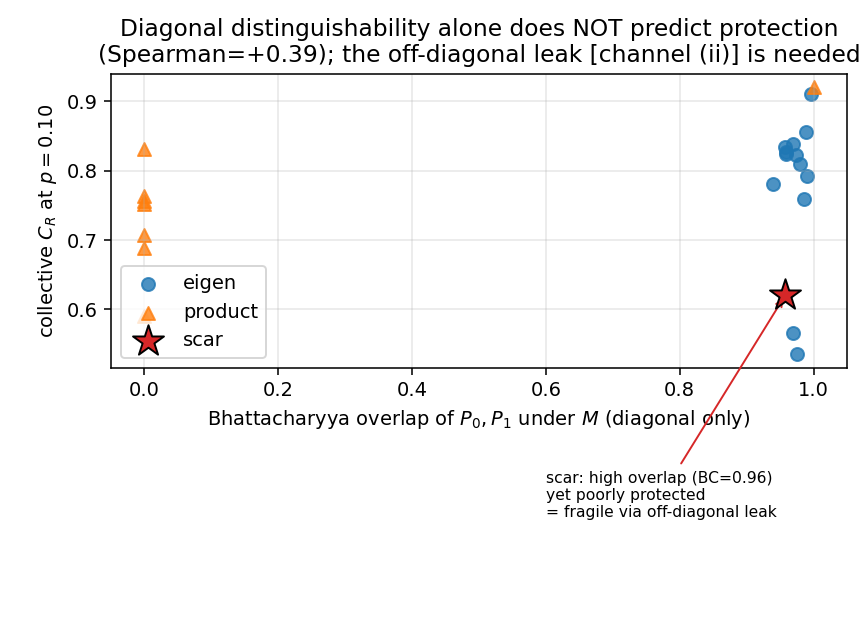
\includegraphics[width=\linewidth]{bhattacharyya.png}
\caption{Collective $\CR$ versus the diagonal Bhattacharyya overlap of the two
logical states under $M$ ($L=14$). The scar (star) has near-unit overlap yet low
$\CR$: its fragility is off-diagonal [channel (ii)], invisible to $\mathrm{BC}$.}
\label{fig:supp_bc}
\end{figure}

\section{Measurement-support phase diagram}
\label{app:phasediagram}

Figure~\ref{fig:supp_pd} maps $\Delta\CR(p,\ell)$ where $\ell$ is the support
size of a block-sum measurement $\sum_{i\in W}Z_i$ over a random contiguous
window $W$ of $\ell$ sites ($\ell{=}1$ local, $\ell{=}L$ global uniform), holding
the per-step event count fixed. Against the ensemble thermal baseline it is
negative throughout: the scar code never wins, and the disadvantage deepens with
both $p$ and $\ell$. (The staggered SGA operator of the main text produces a
larger penalty than the uniform-type block sum because the latter has vanishing
logical leak on the scar rungs.)

\begin{figure}[t]
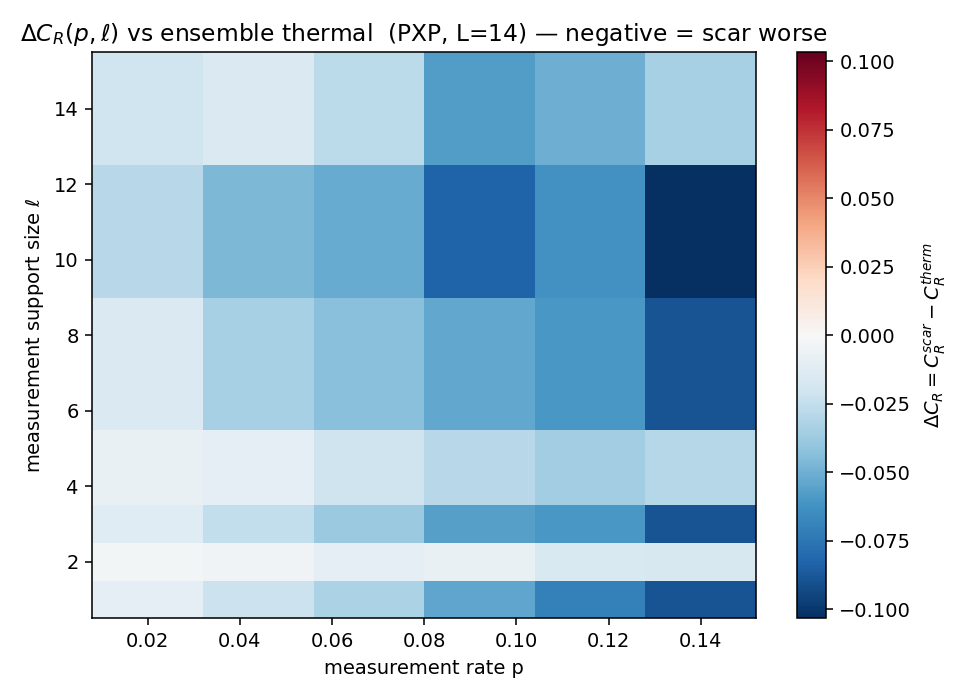
\includegraphics[width=\linewidth]{phase_diagram_L14.png}
\caption{$\Delta\CR(p,\ell)$ against the ensemble thermal baseline (PXP, $L=14$).
Blue is $\Delta\CR<0$ (scar worse) everywhere.}
\label{fig:supp_pd}
\end{figure}

\section{Calibration of the measurement rate}
\label{app:gamma}

To connect our discrete per-step rate to the continuous-time rate of
Ref.~\cite{Paviglianiti2025} we use $\gamma=p/dt$ with $dt=0.6$. An honest
caveat applies: at the sizes and depths accessible here the monitored-N\'eel
entanglement density $S/(L/2)$ decreases with $L$ at \emph{every} $p$
(at $p=0$: $0.285$, $0.258$, $0.241$ for $L=10,12,14$), so the curves in
Fig.~\ref{fig:supp_gamma} do not cross and no volume-law phase---hence no
critical point---is resolved. The minimum of the inter-size spread of
$S/(L/2)$ sits at $p\simeq0.05$ ($\gamma\simeq0.083$), but nearby rates give
almost the same spread ($0.0051$ at $p=0.05$ versus $0.0071$--$0.0072$ at
$p=0.10$--$0.14$), so we treat this only as the scale of steepest variation.
It is of the same order as the reported $\gamma_c\simeq0.013\pm0.002$; we do
not attempt a quantitative comparison of critical rates.

\begin{figure}[t]
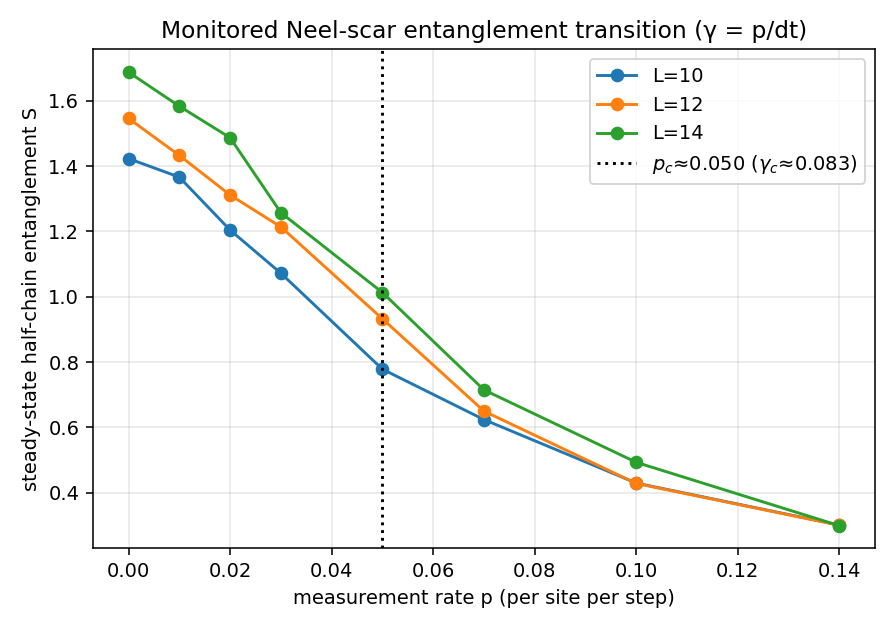
\includegraphics[width=\linewidth]{gamma_mapping.png}
\caption{Half-chain entanglement of the monitored N\'eel state
versus $p$ for $L=10,12,14$. At these sizes and depths the density decreases
with $L$ at every $p$---the curves do not cross---so the marked
$p\simeq0.05$ is the scale of steepest variation, not a critical point.}
\label{fig:supp_gamma}
\end{figure}

\section{Spin-1 Schecter--Iadecola model}
\label{app:spin1}

The second model is the spin-1 chain~\cite{Schecter2019}
\begin{equation}
\begin{split}
H = J\sum_i\!\big(S^x_iS^x_{i+1}+S^y_iS^y_{i+1}\big)
   + h\sum_i S^z_i \\ + D\sum_i (S^z_i)^2,
\end{split}
\end{equation}
with $J{=}1$, $h{=}1$, $D{=}0.1$. Its exact scar tower is
$\ket{S_n}=(Q^+)^n\ket{\Omega}$, $Q^+=\sum_j(-1)^j(S^+_j)^2$,
$\ket{\Omega}=\ket{m{=}{-}1}^{\otimes L}$. The site operators
$\{\ket{m{=}{-}1},\ket{m{=}{+}1}\}$ realize a pseudospin-$\tfrac12$ (with
$\ket{m{=}0}$ outside), and the tower is the fully symmetric Dicke multiplet of
total pseudospin $J=L/2$. With the properly normalized generators
$J^+=Q^+/2$, $J^-=(J^+)^\dagger$, $J^z=\tfrac12\sum_iS^z_i$ one has
$[J^z,J^\pm]=\pm J^\pm$, $[J^+,J^-]=2J^z$, so the Casimir
$J^2=(J^z)^2+\tfrac12(J^+J^-+J^-J^+)$ equals $J(J{+}1)=\tfrac{L}{2}(\tfrac{L}{2}{+}1)$.

We verify numerically that $\ket{S_n}$ are exact eigenstates (residual
$\|H\ket{S_n}-E_n\ket{S_n}\|\sim10^{-16}$), equally spaced by $2$, and that $J^2$
is constant on the tower with variance $\sim10^{-13}$ on every scar---versus
$\mathrm{Var}\,J^2\simeq32$ for PXP scars. Consequently a two-rung scar code has
identical $J^2$ outcome distributions and is an exact decoherence-free subspace
of a $J^2$ measurement, which is why the rescue succeeds here and fails for PXP
($\CR^{\rm scar}=1$, $\Delta\CR=+0.6$ to $+0.9$ at $L=6,8$). Under generic local
$S^z$ monitoring the exact-scar code shows a low-rate advantage whose size
dependence we report in full. At $L=6$ ($20$ pairs)
$\Delta\CR=+0.10,+0.06,-0.02$ at $p=0.04,0.08,0.12$ (ensemble SEM
$\sim0.04$): scar-favorable at the lowest rate (about $2\sigma$), decaying
and reversing sign with $p$, a pattern repeated in two of the three parameter
sets [$(h,D)=(1.5,0.0)$: $+0.11,+0.03,-0.02$; $(0.5,0.3)$:
$+0.05,-0.03,-0.05$]. At $L=8$ ($20$ pairs) the difference is larger and
stays positive across our window: $\Delta\CR=+0.20,+0.10,+0.08$ (ensemble
SEM $0.05$--$0.07$, so $\approx3\sigma$ at $p=0.04$). With two sizes we
cannot settle the large-$L$ fate of this local-measurement advantage; what
the data establish is that it decays with rate, and that the unconditional
scar-versus-thermal reversal seen for PXP does not occur for exact scars.

\section{A single-shot resolvability predictor}
\label{app:predictor}

The two channels of the main-text criterion combine into one exact,
simulation-free scalar: the reference entropy that survives a \emph{single}
projective $O$-measurement of the freshly encoded pair,
\begin{equation}
s_1(O)=\sum_g q_g\, S\!\big(\rho_R^{(g)}\big),\qquad
\big[\rho_R^{(g)}\big]_{ab} = \frac{\langle b_L|\Pi_g|a_L\rangle}{2q_g},
\end{equation}
with $\Pi_g$ the spectral projectors of $O$ and $q_g=\tfrac12(\langle
0_L|\Pi_g|0_L\rangle+\langle1_L|\Pi_g|1_L\rangle)$ the Born weights. By
construction $s_1=1$ iff a single shot leaves the qubit perfectly
recoverable---the Knill--Laflamme conditions for the projector set
$\{\Pi_g\}$, of which a common-eigenvalue eigenspace (a true DFS) is the
simplest realization---and $s_1=0$ iff one shot fully reads the qubit out;
eigenvalue distinguishability [channel (i)] and non-invariance [channel (ii)]
both enter automatically.

Across $65$ code--measurement pairs spanning both models and five global
operators (Fig.~\ref{fig:supp_pred}), $s_1$ strongly predicts the monitored
$\CR$ \emph{within each resolving measurement}: Spearman $\rho=+0.84$ (PXP,
staggered), $+0.87$ and $+0.79$ (spin-1, Casimir and staggered). Two
limiting behaviors delimit its scope and are themselves instructive: for a
non-resolving operator (PXP uniform, $s_1\approx1$ for all codes) there is no
signal left to predict ($\rho=-0.09$, $p=0.75$), and for an operator that
does not commute with the Hamiltonian (the PXP Casimir, $[J^2,H]\neq0$) the
ranking survives ($\rho=+0.69$, $p=0.004$) but the dynamics between shots
dress the resolvability and shift $\CR$ systematically below the single-shot
estimate. We therefore present $s_1$ as an operational design quantity---an
exact, Monte-Carlo-free screen for candidate code/measurement pairs---rather
than a universal collapse variable.

\begin{figure}[t]
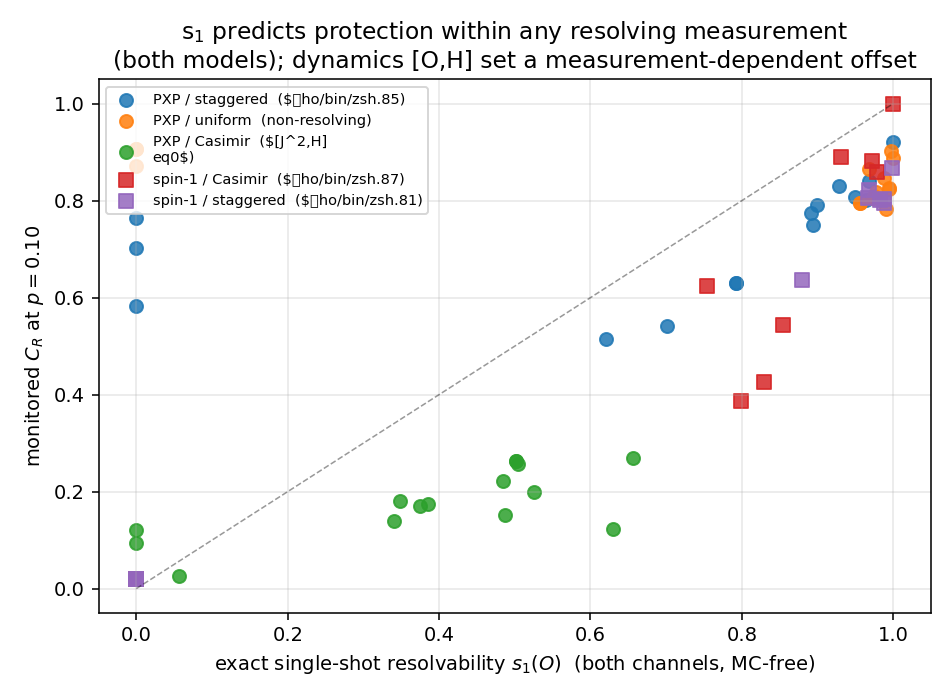
\includegraphics[width=\linewidth]{predictor.png}
\caption{Monitored $\CR$ ($p=0.10$) versus the exact single-shot resolvability
$s_1(O)$ for $65$ code--measurement pairs across both models. Within each
resolving measurement the relation is tight; the non-resolving (uniform) and
non-commuting (PXP Casimir) families bound the predictor's scope.}
\label{fig:supp_pred}
\end{figure}

\section{Extensive code under collective and Casimir monitoring}
\label{app:extensive}

The maximal $k=\lfloor\log_2(L{+}1)\rfloor$-qubit scar code of the main text is
compared to a same-dimension thermal code under all three PXP measurement models
in Table~\ref{tab:ext} ($L=14$, $k=3$, protected density $S_R/k$, $8$-draw
thermal ensemble). The pattern matches the single-qubit analysis: the scar loses
under local and (strongly) collective monitoring and is only comparable
(marginally scar-favorable, within $\lesssim0.03$) under the fine-tuned
Casimir---the one measurement model in which the thermal code does not win.
The local run used the grid $p=0,0.02,0.04,0.08$ of Fig.~\ref{fig:ext} (its
$p=0.02$ gap is $-0.17$); the collective and Casimir runs used
$p=0,0.04,0.08,0.12$, hence the ragged table.

Two selection details deserve disclosure. The $2^k$ code states are the
tower states of largest $\Ztwo$ overlap, which at $L=14$ comprise six
$\pm E$ rung partners, the $E=4.06$ rung, and one $E\simeq0$ tower state;
the positive-rung restriction of the single-qubit analysis
(Appendix~\ref{app:spectrum}) is not imposed, since $2^k=8$ exceeds the six
positive rungs available. Excluding the zero mode entirely (selecting the
top-$8$ among tower states with $|E|>0.8$) changes nothing: the local
densities move from $0.674/0.393/0.101$ to $0.661/0.381/0.104$ at
$p=0.02/0.04/0.08$, both far below the thermal $0.83/0.55/0.17$
(\texttt{scripts/referee\_audit.py}).

\begin{table}[h]
\caption{Extensive-code density gap $\Delta(S_R/k)=$ scar $-$ thermal ($L=14$,
$k=3$).}
\label{tab:ext}
\centering
\begin{tabular}{lccc}
\toprule
measurement & $p{=}0.04$ & $p{=}0.08$ & $p{=}0.12$ \\
\midrule
local $S^z$    & $-0.14$ & $-0.06$ & --- \\
collective $M$ & $-0.32$ & $-0.40$ & $-0.43$ \\
Casimir $J^2$  & $+0.02$ & $+0.03$ & $+0.03$ \\
\bottomrule
\end{tabular}
\end{table}

\bibliographystyle{quantum}
\bibliography{../refs}

\end{document}
